\chapter{Página Inicial}
\label{chap:paginaInicial}

\section{Padrão de endereço do noosfero}
\label{sec:padraoEndereco}

Os endereços das páginas da plataforma Noosfero tem o seguinte padrão

\begin{table}[h]
\begin{tabular}{|l|l|}
  \hline
  \multicolumn{1}{|c|}{\textbf{Endereço}} & \multicolumn{1}{c|}{\textbf{Destino}} \\
  \hline
  \textbackslash & Página Inicial \\
  \textbackslash nome-comunidade & Comunidade \\
  \textbackslash nome-comunidade\textbackslash nome-conteudo & Conteúdo dentro de uma comunidade \\
  \hline
\end{tabular}
\caption {Padrão de Endereços}
\end{table}

\section{Definindo Página Inicial}
\label{sec:paginaInicial}

\section{Menu superior}
\label{menuSuperior}
\begin{figure}[h]
     \centering
       
\includegraphics[keepaspectratio=true,scale=0.49]{figuras/menu_superior}
     \caption{Menu superior}
\end{figure}

O menu superior é um dos poucos conteúdos no Noosfero que deve ser alterado 
diretamente pelo arquivo fonte. No entanto, não é uma tarefa árdua, muito pelo
contrário.

\newpage
\subsection{Entendendo a estrutura do menu}

Acessando o arquivo \emph{\textbf{noosfero/public/designs/themes/portalCpd/header.html.erb}},
deverá ser editado a seção \emph {\textbf{menu-top}}.

\begin{figure}[h]
     \centering
       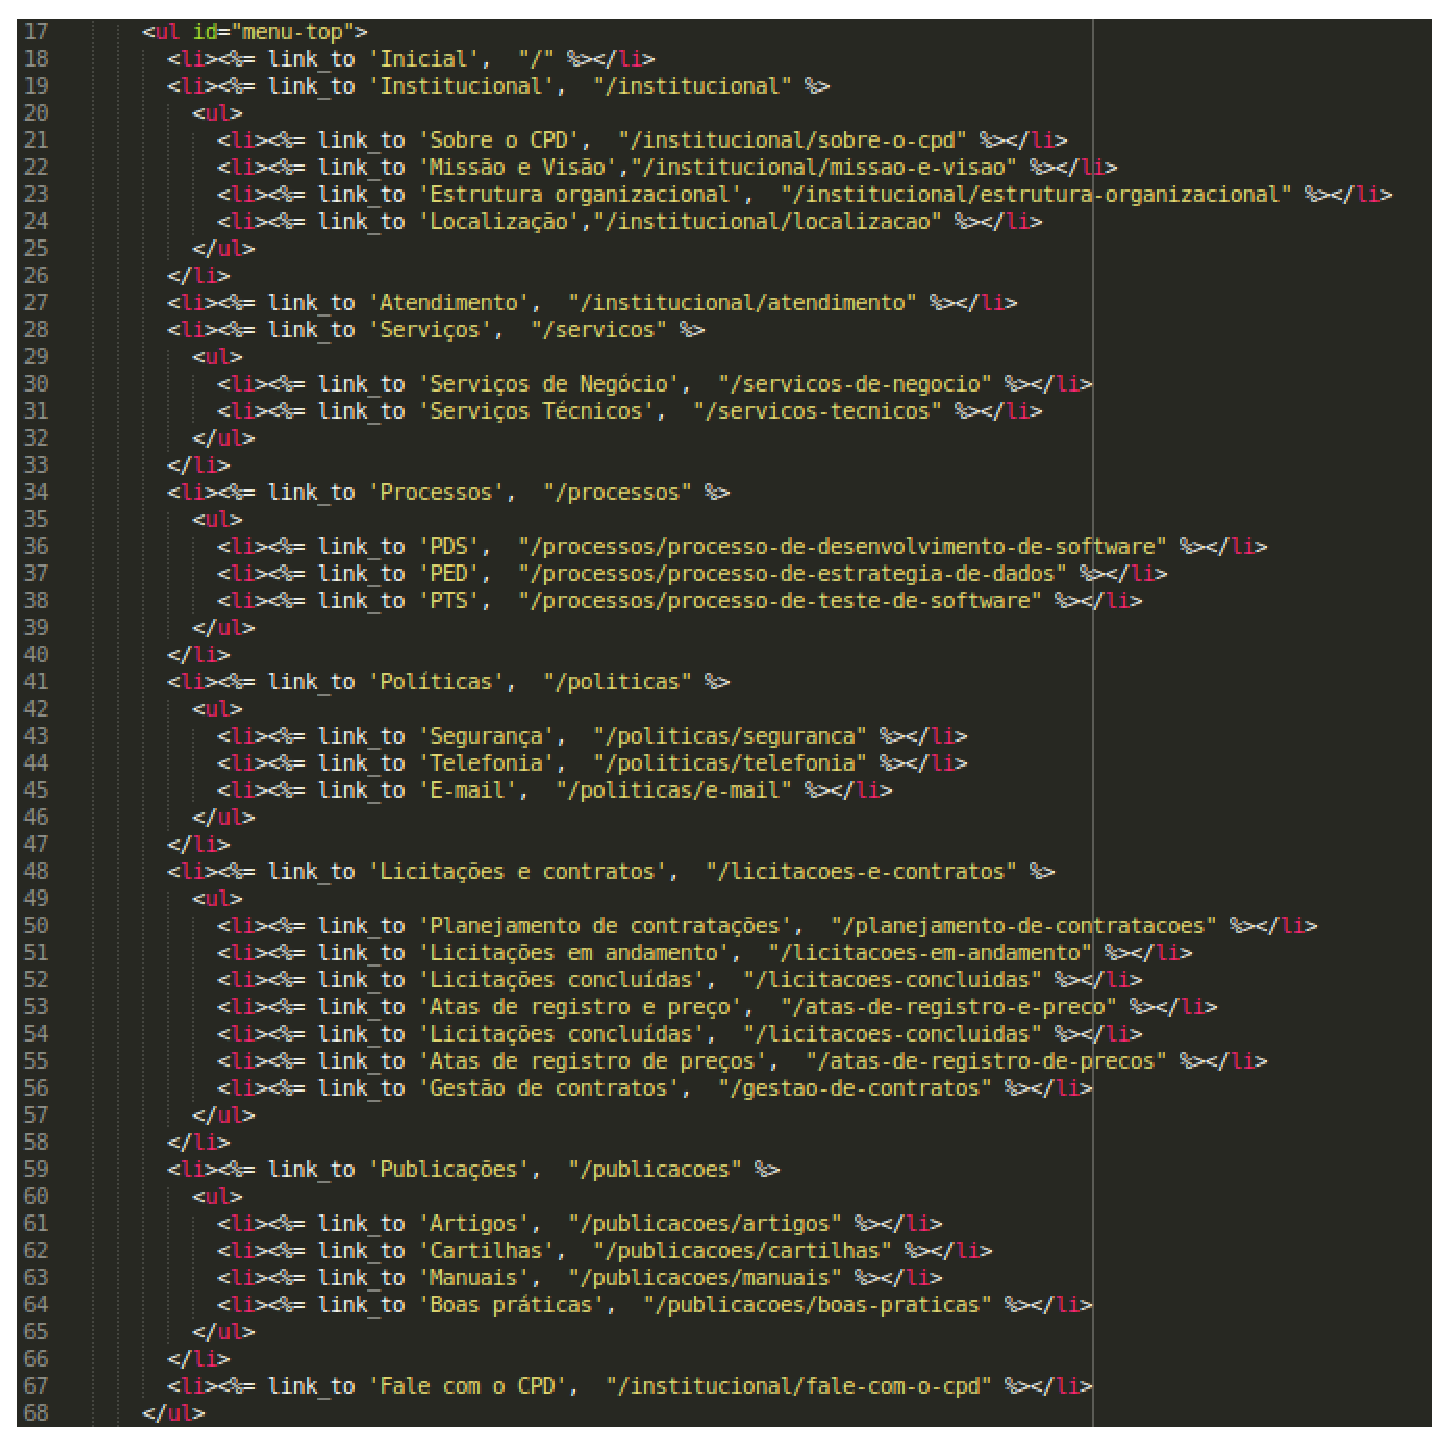
\includegraphics[scale=0.5]{figuras/menu-top}
     \caption{Arquivo de Configuração do Menu Superior}
     \label{fig:configMenuSuperior}
\end{figure}

Repare na \ref{fig:configMenuSuperior}, que as linhas mais próximas da borda esquerdo da imagem, são os itens do menu, e as linhas mais distantes da borda esquerda são os sub-itens do menu.

Para ficar mais claro, as linhas 18, 19, 27, 28, 34, 41, 48, 59, e 67 são itens do menus, e as linhas 21, 22, 23, 24, 30, 31, 36, 37, 38, 43, 44, 45, 50, 51, 52, 53, 54, 55, 56, 61, 62, 63, 65 são sub-itens do menu.

Os itens e sub-itens do menu possuem a mesma estrutura:

\begin{minted}[
  frame=single
]{erb}
<%= link_to 'Nome do item/subitem', "/endereco-da-pagina" %>
\end{minted}

Consulte a seção \ref{sec:padraoEndereco} para conhecer o padrão de endereço utilizado pelo Noosfero.

\newpage
\subsection{Adicionando um item a estrutura do menu}

O menu superior tem uma estrutura básica, mostrada no Exemplo 1:

\begin{minted}[
  frame=single,
  label=Exemplo 1
]{erb}
<li><%= link_to 'Item 1 (com sub-itens)', "/endereco" %><\li>
  <ul>
    <li><%= link_to 'Subitem 1', "/endereco-da-pagina" %><\li>
    <li><%= link_to 'Subitem 2', "/endereco-da-pagina" %><\li>
  </ul>
<li><%= link_to 'Item 2 (sem subitem)', "/endereco-da-pagina" %><\li>
\end{minted}

Caso deseje acrescentar um item ao menu do Exemplo 1, basta adicionar:

\begin{minted}[
  frame=single
]{erb}
<li><%= link_to 'Novo Item', "/endereco-da-pagina" %></li>
\end{minted}

O arquivo ficará:

\begin{minted}[
  frame=single,
  label=Exemplo 2
]{erb}
<li><%= link_to 'Item 1 (com sub-itens)', "/endereco" %><\li>
  <ul>
    <li><%= link_to 'Subitem 1', "/endereco-da-pagina" %><\li>
    <li><%= link_to 'Subitem 2', "/endereco-da-pagina" %><\li>
  </ul>
<li><%= link_to 'Item 2 (sem subitem)', "/endereco-da-pagina" %><\li>
<li><%= link_to 'Novo Item', "/endereco-da-pagina" %></li>
\end{minted}

Consulte a seção \ref{sec:padraoEndereco} para conhecer o padrão de endereço utilizado pelo Noosfero.

\subsection{Adicionando um subitem}

A adição de um subitem é um pouco mais complicada. Caso se deseje acrescentar um subitem a um item do menu que já passua um subitem, como é o caso do Item 1 do Exemplo 2, basta adicionar, de forma análoga a adição de um item, a seguinte linha:

\begin{minted}[
  frame=single
]{erb}
    <li><%= link_to 'Novo subitem 3', "/endereco-da-pagina" %></li>
\end{minted}

\newpage
Ficará assim:

\begin{minted}[
  frame=single,
  label=Exemplo 3
]{erb}
<li><%= link_to 'Item 1 (com sub-itens)', "/endereco" %><\li>
  <ul>
    <li><%= link_to 'Subitem 1', "/endereco-da-pagina" %><\li>
    <li><%= link_to 'Subitem 2', "/endereco-da-pagina" %><\li>
    <li><%= link_to 'Novo subitem 3', "/endereco-da-pagina" %></li>
  </ul>
<li><%= link_to 'Item 2 (sem subitem)', "/endereco-da-pagina" %><\li>
<li><%= link_to 'Novo Item', "/endereco-da-pagina" %></li>
\end{minted}

Para adicionar um subitem a um menu que não possui sub-itens, como é o caso do Item 2 do Exemplo 3, deverá ser adicionado a seguinte estrutura:

\begin{minted}[
  frame=single,
]{erb}
  <ul>
    <li><%= link_to 'Novo subitem 4', "/endereco-da-pagina" %><\li>
  </ul>
\end{minted}

Ficará assim:

\begin{minted}[
  frame=single,
  label=Exemplo 4
]{erb}
<li><%= link_to 'Item 1 (com sub-itens)', "/endereco" %><\li>
  <ul>
    <li><%= link_to 'Subitem 1', "/endereco-da-pagina" %><\li>
    <li><%= link_to 'Subitem 2', "/endereco-da-pagina" %><\li>
    <li><%= link_to 'Novo subitem 3', "/endereco-da-pagina" %></li>
  </ul>
<li><%= link_to 'Item 2 (sem subitem)', "/endereco-da-pagina" %><\li>
  <ul>
    <li><%= link_to 'Novo subitem 4', "/endereco-da-pagina" %></li>
  </ul>
</li>
<li><%= link_to 'Novo Item', "/endereco-da-pagina" %></li>
\end{minted}

Consulte a seção \ref{sec:padraoEndereco} para conhecer o padrão de endereço utilizado pelo Noosfero.

\newpage
\section{Rodapé}

\begin{lstlisting}
$ /usr/share/noosfero\label{sec:greetings}
\end{lstlisting}

Assim como o menu superior na seção \ref{menuSuperior}, o rodapé da página também deve ser alterado no arquivo de código fonte. Para isso acesse o arquivo \textbf{\textit{noosfero/public/designs/themes/portalCpd/footer.html.erb}}

A figura abaixo mostra como está a estrutura do rodapé da página.
\begin{figure}[h]
     \centering
       
\includegraphics[keepaspectratio=true,scale=0.49]{figuras/footer.eps}
     \caption{Rodapé da página.}
\end{figure}

Percebe-se que há um conjunto de \emph{links} que possibilitam o acesso rápido às informações (Página Inicial, Sobre, Contato), para realizar o acréscimo ou alteração de alguma informação o procedimento é semelhante ao menu superior basicamente o código utilizado é:

\begin{lstlisting}
<li><%= link_to '< Menu a ser adicionado >',  "< Link de acesso >" %></li>
\end{lstlisting}

Quando definido tais parâmetros eles devem ser adicionados ao código no arquivo \emph{footer.html.erb} e ficará conforme a figura \ref{fig:codMenu}:

\begin{figure}[h]
     \centering
       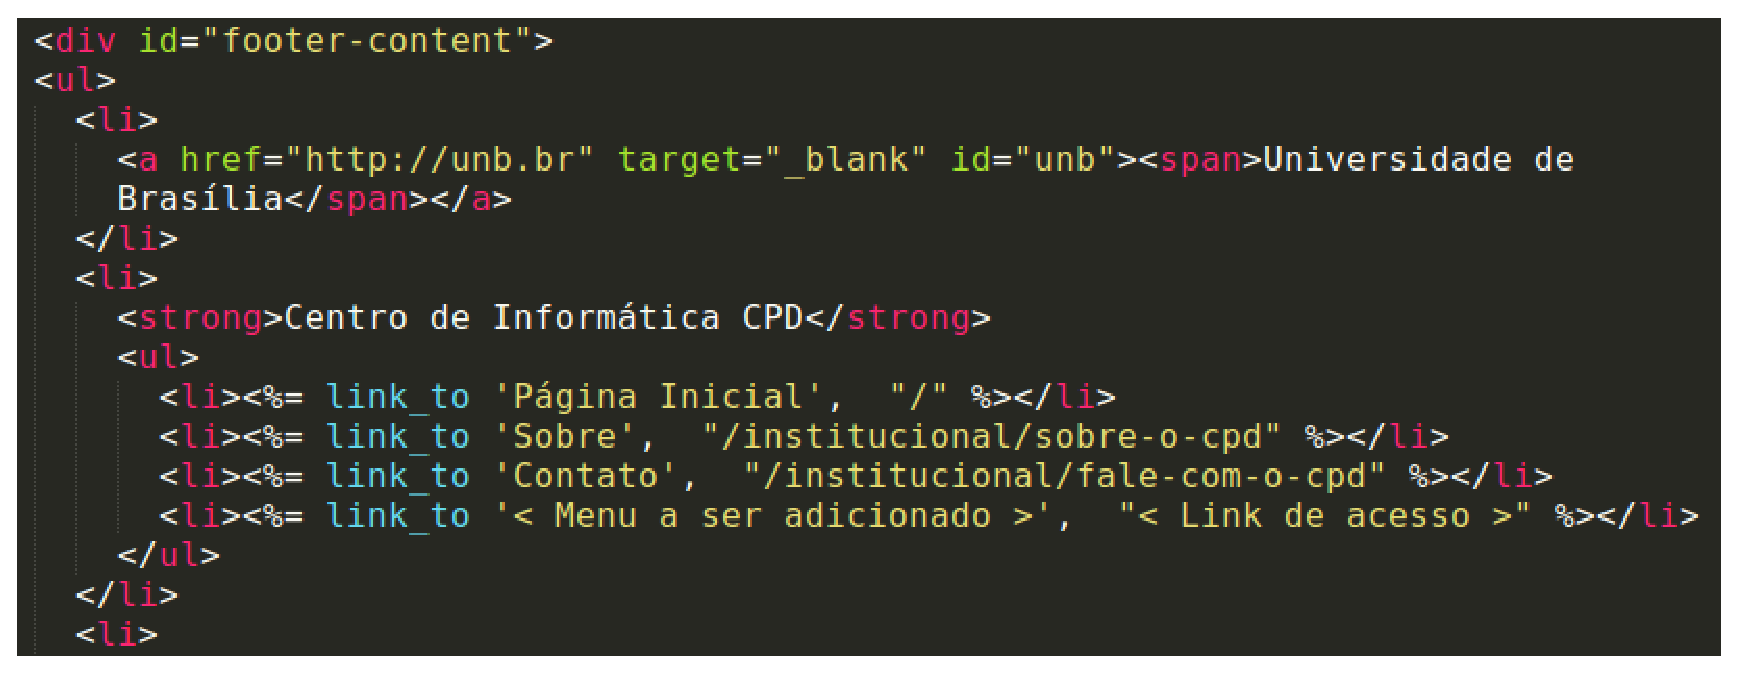
\includegraphics[keepaspectratio=true,scale=0.3]{figuras/footerMenu.eps}
     \caption{Código do menu da página.}
     \label{fig:codMenu}
\end{figure}

\newpage
Para adicionar informações gerais referentes ao portal deve ser alterado o conteúdo dentro da \emph{<div id='license-on-footer'>}, segue abaixo a figura \ref{fig:infGeral} que contém todas as informações referentes ao portal do CPD.

\begin{figure}[h]
     \centering
       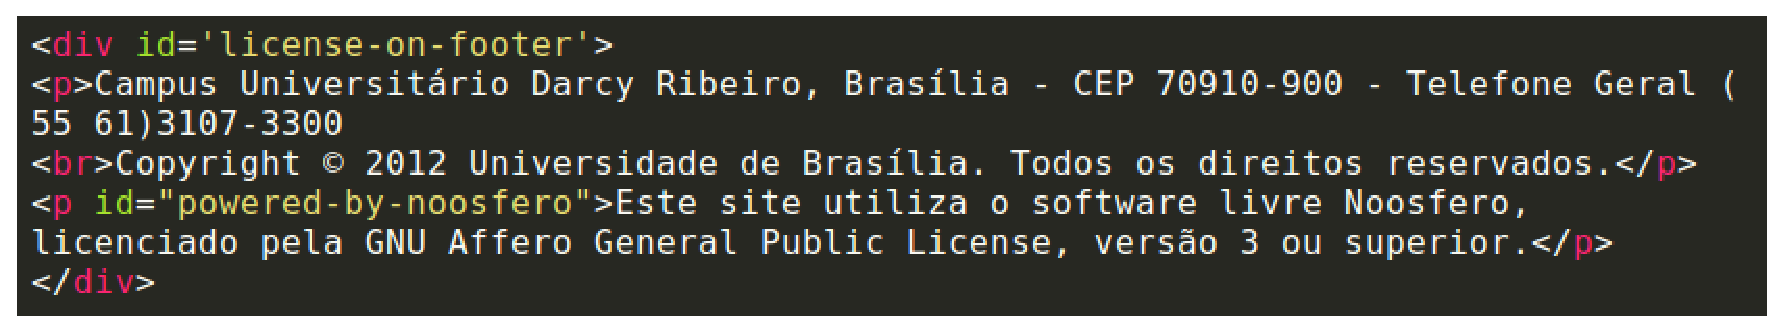
\includegraphics[keepaspectratio=true,scale=0.49]{figuras/informacoesGeraisRodape.eps}
     \caption{Informações gerais.}
     \label{fig:infGeral}
\end{figure}

Consulte a seção \ref{sec:padraoEndereco} para conhecer o padrão de endereço utilizado pelo Noosfero.

\section{Menu lateral}

Para a edição do menu lateral é necessário entrar no painel de controle administrativo do Noosfero. Então, vá até o rodapé do site e clique no link \emph{\color{red}Administração}.

\begin{figure}[h]
     \centering
       
\includegraphics[keepaspectratio=true,scale=0.6]{figuras/linkAdmin.eps}
     \caption{Link para a Administração do site.}
     \label{fig:linkAdmin}
\end{figure}

\newpage
Dentro do painel de controle administrativo, clique em \emph{\color{red}Blocos laterais}.

\begin{figure}[h]
     \centering
       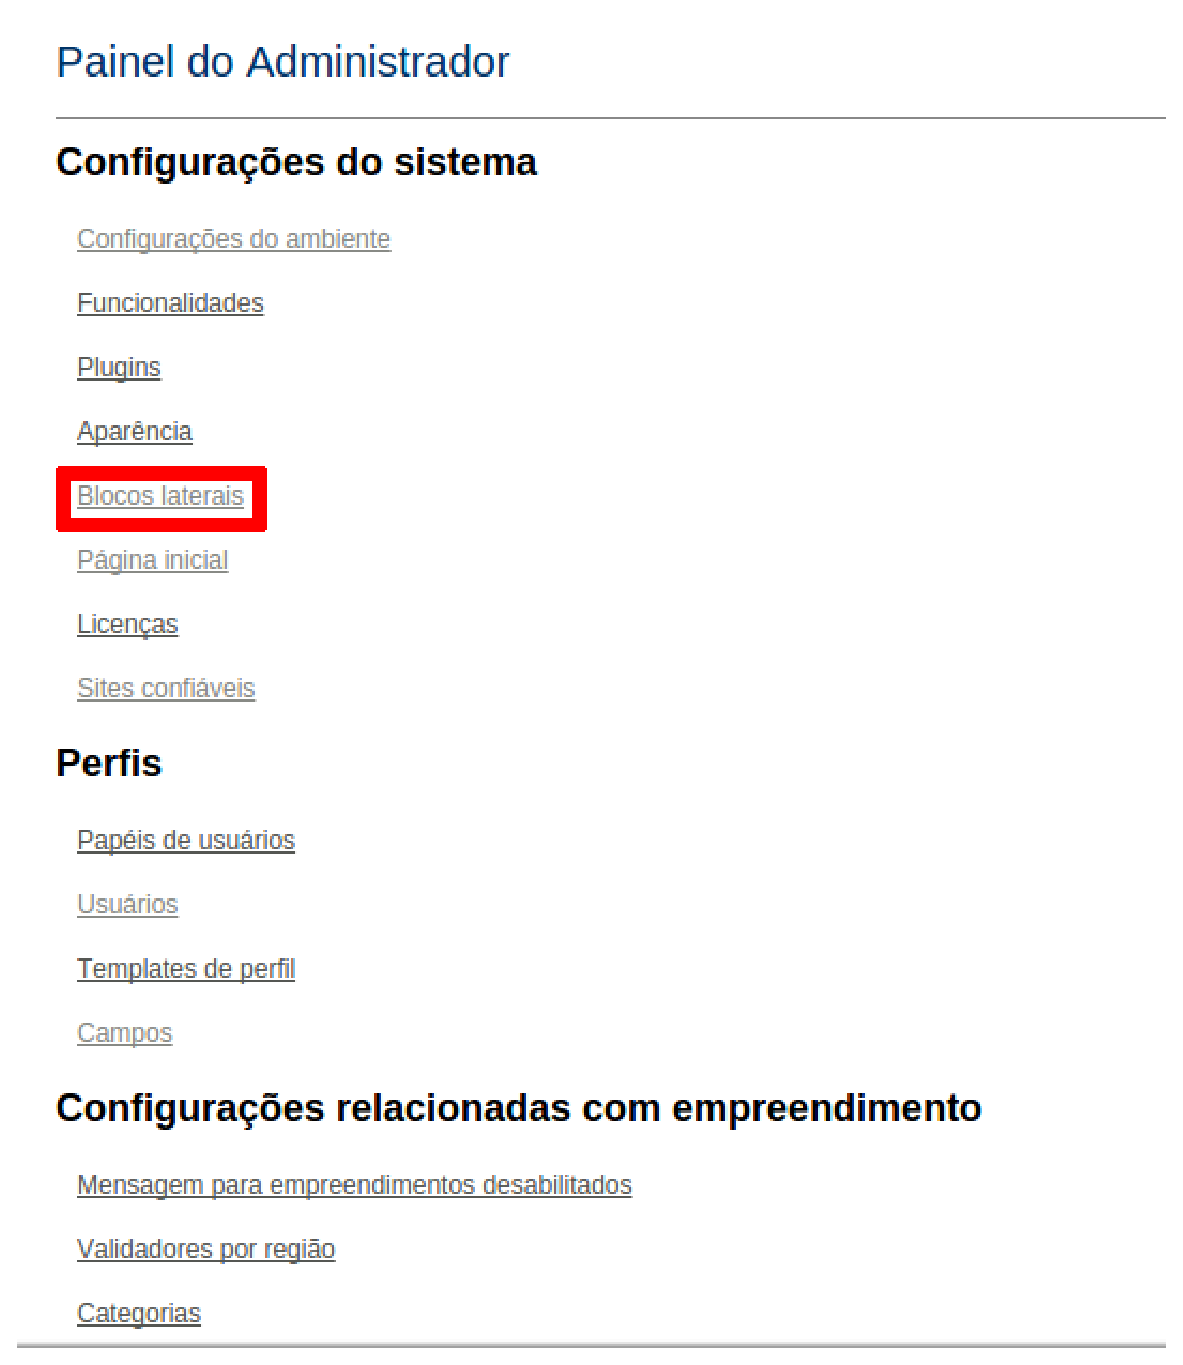
\includegraphics[keepaspectratio=true,scale=0.4]{figuras/administracao.eps}
     \caption{Painel de Controle Administrativo.}
     \label{fig:painelAdministrativo}
\end{figure}

Posicione o mouse em cima do \emph{\color{red}menu lateral} e clique no ícone \emph{\color{green}Editar}.

\begin{figure}[h]
     \centering
       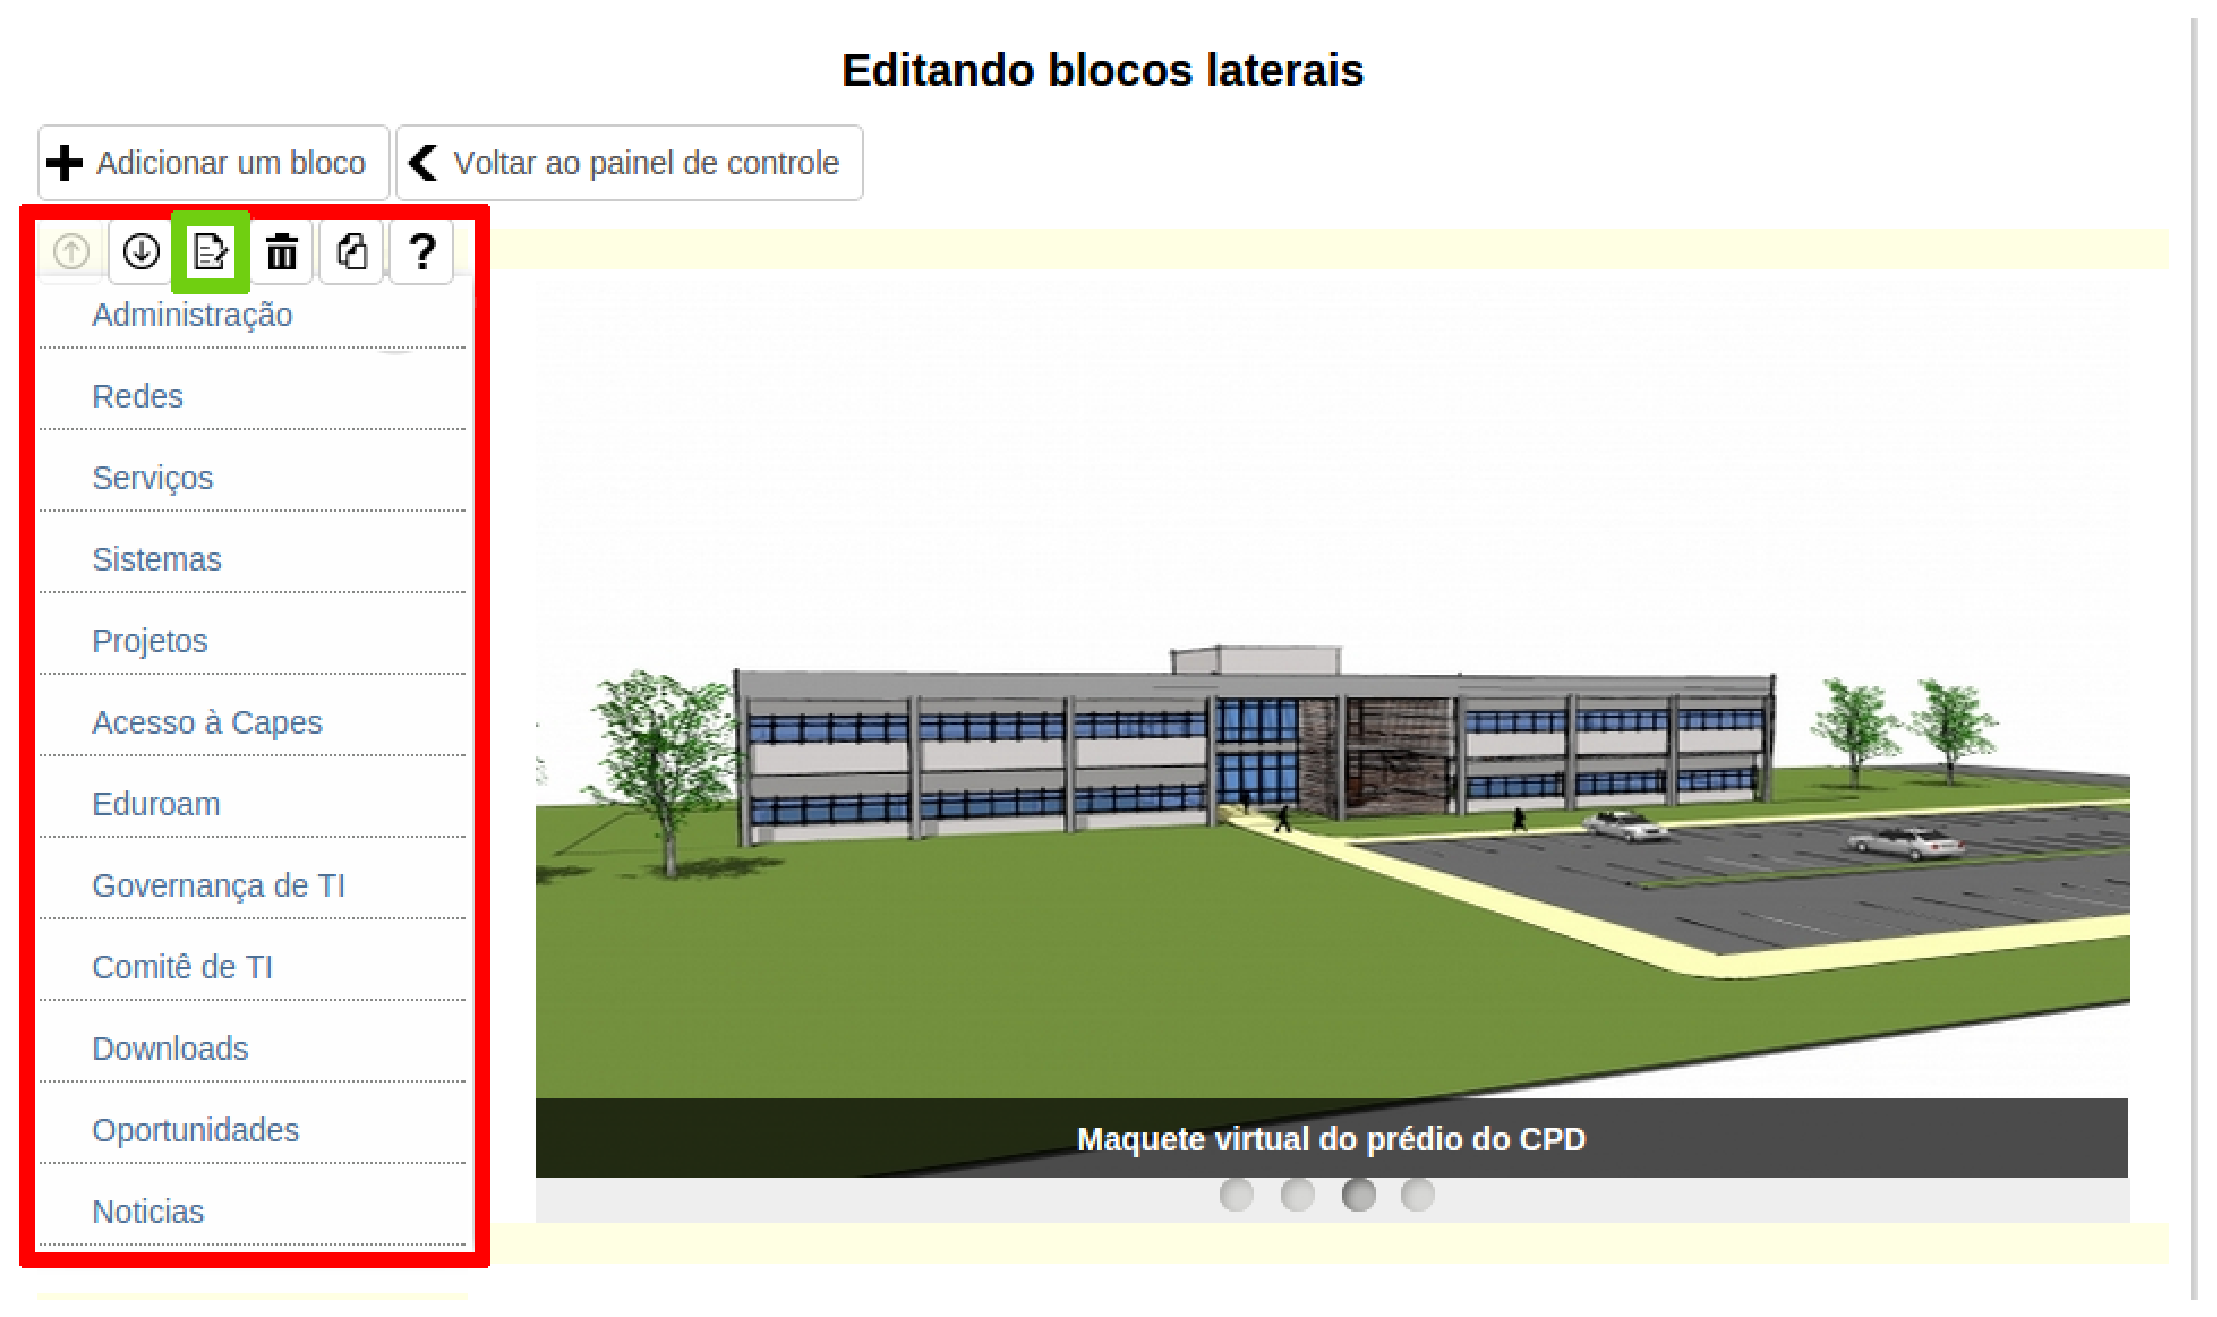
\includegraphics[keepaspectratio=true,scale=0.4]{figuras/editarBlocoLateral.eps}
     \caption{Editar Bloco Lateral.}
     \label{fig:editarBloco}
\end{figure}

\newpage
Na tela de edição do menu lateral, podemos adicionar um novo item ao menu clicando em \emph{\color{red}Novo Link}. No primeiro campo adicione o nome do novo item do menu, e no segundo campo, o endereço do mesmo.

Consulte a seção \ref{sec:padraoEndereco} para conhecer o padrão de endereço utilizado pelo Noosfero.

Caso deseje remover um item do menu, clique no botão \emph{\color{orange}Remover}.

Clique no \emph{\color{yellow}Ícone} para modificar o ícone mostrado ao lado do nome do item do menu.

Você também pode alterar a ordem dos itens pressionando o botão esquerdo do mouse em cima do item do menu e o arrastando-o para onde desejar. 
\textbf{PS: O \emph{\color{blue}ícone de movimentação} irá aparecer quando você estiver com o mouse posicionado em cima do item do menu.}

\begin{figure}[h]
     \centering
       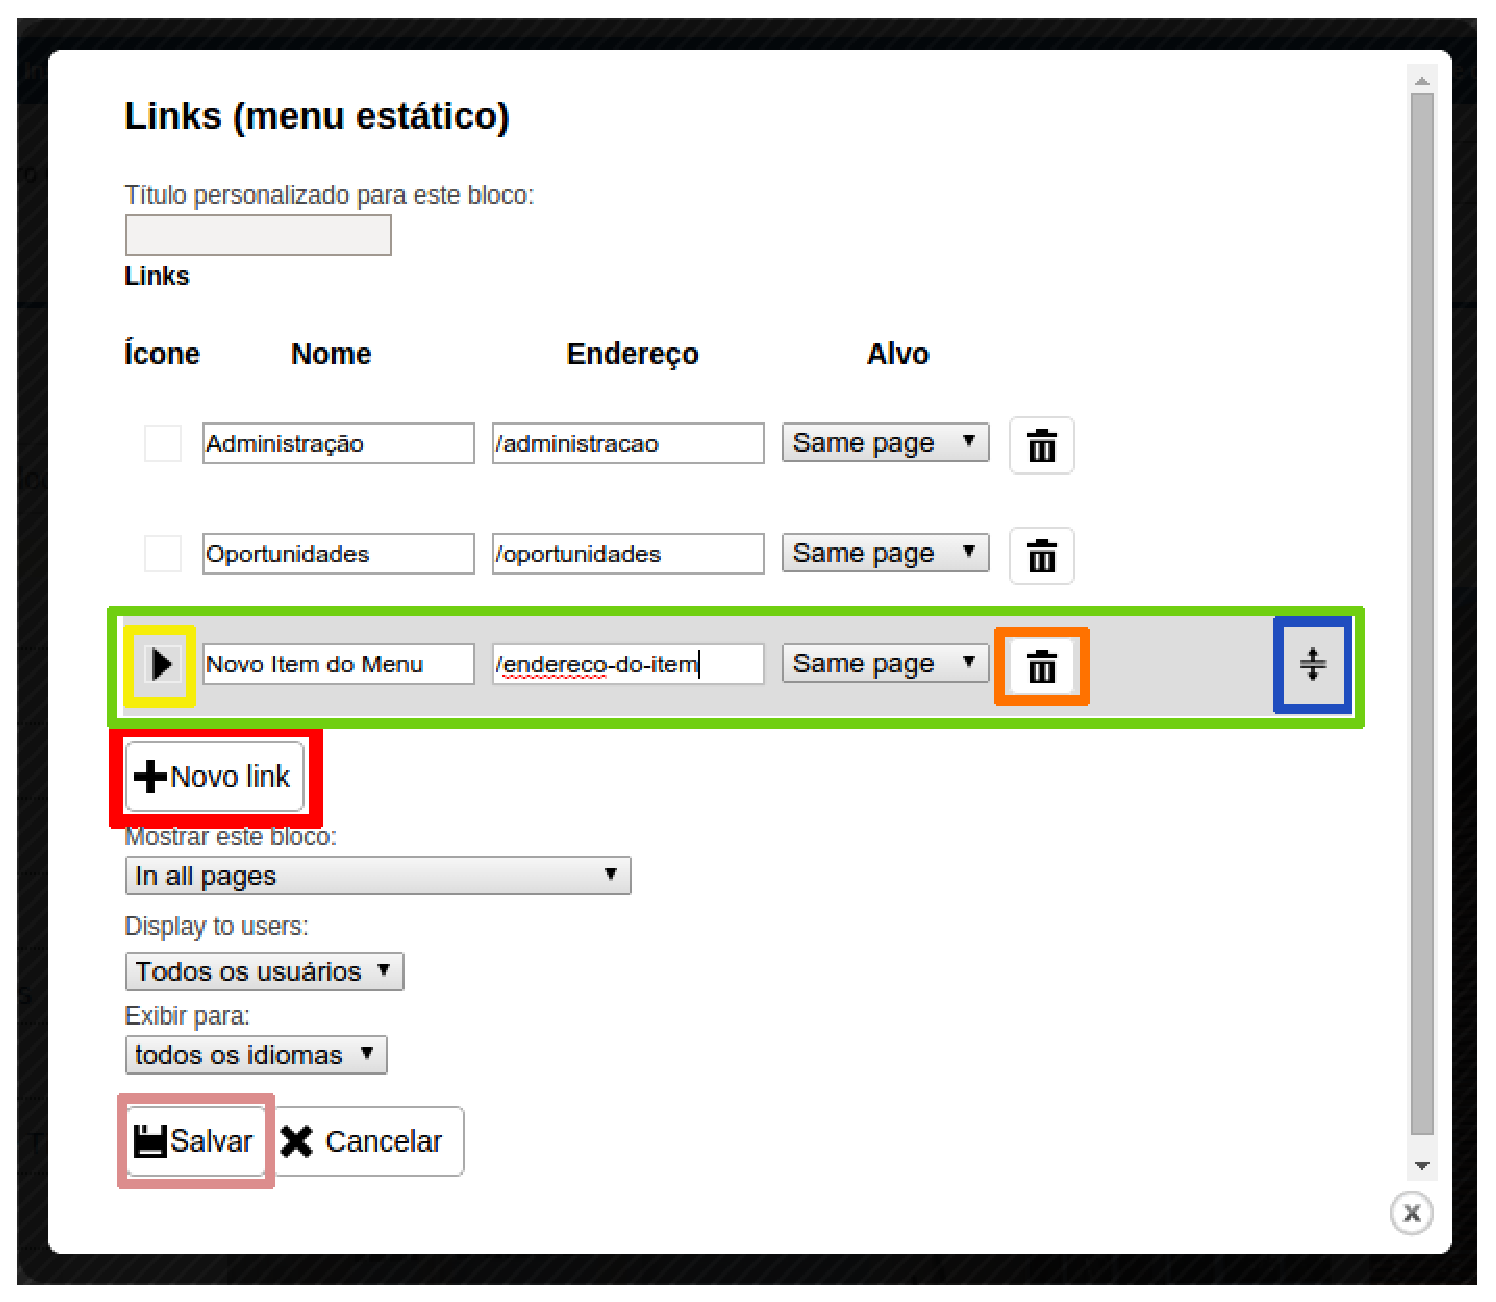
\includegraphics[keepaspectratio=true,scale=0.4]{figuras/editarMenuLateral.eps}
     \caption{Editar menu lateral.}
     \label{fig:editarMenuLateral}
\end{figure}
